\documentclass[a4paper]{article}
\usepackage{graphicx}
\usepackage{url}
\usepackage{twocolpceurws}

\title{From Python to Pythonic:\\ Searching for Python idioms in GitHub}

\author{
Jos\'e Javier Merchante
 \\ 
Universidad Rey Juan Carlos\\
Fuenlabrada, Madrid, Spain\\
Email: jj.merchante@gmail.com
\and
Gregorio Robles \\ GSyC/LibreSoft\\
Universidad Rey Juan Carlos\\
Fuenlabrada, Madrid, Spain\\
Email: grex@gsyc.urjc.es
}

\institution{}

\begin{document}

\maketitle

\begin{abstract}
    This paper presents our work in progress. Our study is focused on creating a web tool that can help beginners and advanced programmers to make their Python code more legible and readable with the use of Pythonic idioms, that is, using typical ways to accomplish some tasks.
\end{abstract}

\section{Introduction}

Every programming language has its culture and usual way to code a task; that's what programmers usually call \emph{idioms}~\cite{coplien1997advanced}. For an advanced programmer in a given language there is always a \emph{better} way of accomplishing a task that is more suitable in that language (e.g., it improves its readability) instead of writing the implementation it replaces in the same way as in another language.

Python is a programming language that in the last years has grown a lot. For this language there are many tools that check the code against very common style conventions (such as the ones specified in the PEP-8\footnote{PEP 8 -- Style Guide for Python Code: https://www.python.org/dev/peps/pep-0008/.}), but there is to our knowledge no tool that identifies what idioms a program contains, or that helps improving your Python code making it more idiomatic (commonly referred to as more \emph{Pythonic}~\cite{van2007python}). Even though no such tool exist, the Python community is concerned a lot about these issues and many books, articles, talks and references on how to make your Python code more Pythonic can be found.

Many Python books and web pages explain the language without including these idioms, and focus on explaining the language as it would be another programming language, but with Python syntax. As an example, the following is correct Python:

\begin{verbatim}
colors = ["blue", "red", "yellow"]

for i in range(len(colors)):
    print colors[i]
\end{verbatim}

However, even if the code runs and works perfectly, there is a more \emph{Pythonic} way of
doing it:

\begin{verbatim}
colors = ["blue", "red", "yellow"]

for color in colors:
    print color
\end{verbatim}

For these reasons, we think it would be a good idea to analyze Python idioms and create a web application that can help beginners and advanced programmers to make their Python code more legible, readable, and write the task the \emph{right}, \emph{Pythonic} way.

\section{Methodology}

For the implementation of this tool we have searched for the most important Python idioms in books and talks at PythonCon, the most important conference on Python. Like this, we have collected Python idioms of various difficulty levels. This list contains idioms such as: List comprehensions, magic methods, lambda functions, decorators, collections structures, class methods or closures.

In order to identify the idioms in Python source code, we look for tokens in Python code. For some idioms, this is straightforward (e.g., for the \emph{with} keyword), while for others it is more complex (e.g., for list comprehensions, in particular those that contain Boolean logic). Then, we scan Python code in a project with a lexer called \texttt{Pygments}\footnote{http://pygments.org/} for these idioms.

For each idiom found, we also retrieve and store meta-information from the versioning repository, such as its author (we therefore use \texttt{git blame}). That allows to obtain the Pythonic contribution of each collaborator to a GitHub project.

In order to improve our tool and to perform a first study of the use of Pythonic elements in real Python code, we mined all projects with Python as main language from GitHub. We used GHTorrent~\cite{gousios2012ghtorrent} as data source for knowing the main programming language of a repository\footnote{We do only consider those repositories that are non-forks.}, of which 700,000 (out of over 15 million) were in Python. Out of these, we downloaded a sample of 70,000 projects.

Given the amount of data to be downloaded and analyzed, the analysis of the repositories took five weeks. Projects were downloaded, and then non-Python files in them were removed in order to store space. All in all, at the end of the process we had a total of 500 GB of Python files. These were analyzed with our tool. The output was redirected to a database and analyzed with Pandas~\cite{mckinney2012python}.

\section{Some preliminary results}

In this section, we present some preliminary results. 

Figure~\ref{fig:idioms_per_repository} shows the number of idioms per repository. This curve shows a powerlaw distribution with a long tail: many of the repository have few idioms, although more than 50\% of the repositories have more than 40 idioms -- the mean is 304.52. Noteworthy is the fact that around 12\% of the repositories do not contain any of the Python idioms in their code.

\begin{figure}[ht]
\centering  
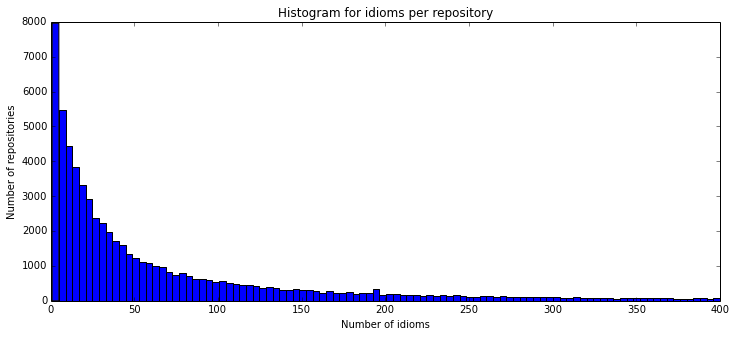
\includegraphics[width=82mm]{img/idioms_per_repository.png}
\caption{Number of idioms per repository}
\label{fig:idioms_per_repository}
\end{figure}


Figure~\ref{fig:idiom_ranking} displays the most used idioms by number of repositories, counting an idiom only once per repository. As can be observed, decorators and list comprehensions are two of the most common Python idioms, although the most frequent ones are the use of named arguments in function calls and \emph{docstrings} (attached comments in a specific format that serves as documentation for classes and methods). The \verb|if __name__ == "__main__"| construct is also at least one time in a repository for over 80\% of the cases.

\begin{figure}[ht]
\centering
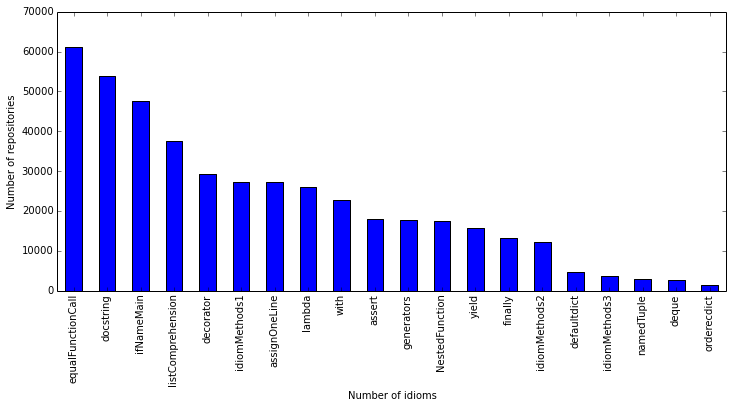
\includegraphics[width=82mm]{img/num_idiom_repo.png}
\caption{Ranking of most frequent Python idioms. Idioms are counted only once per repository.}
\label{fig:idiom_ranking}
\end{figure}

Some of the most used and known Python idioms are \emph{magic} methods (methods that are invoked when using a certain syntax, starting and finishing with \_\_, also known as \emph{dunder} from \emph{double under}). These methods provide characteristics that, if implemented, are \emph{transversal} to classes and thus provide a common, defined way for some functionality. An example of this are the \_\_repr\_\_, which returns a printable representation of an object, and \_\_str\_\_, which returns a string containing a nicely printable representation of an object, methods. Figure~\ref{fig:magic_ranking} gives the number of occurrences of each of the most frequent magic methods. This time, the total number of appearances, i.e., a magic method that appears N times in a repository will count N for that repository, is given. The most frequent one, \verb|__init__| (the initializer method, used in Python in a constructor-ish nature), is omitted in the figure as it appears many more times than the rest.

\begin{figure}[ht]
\centering
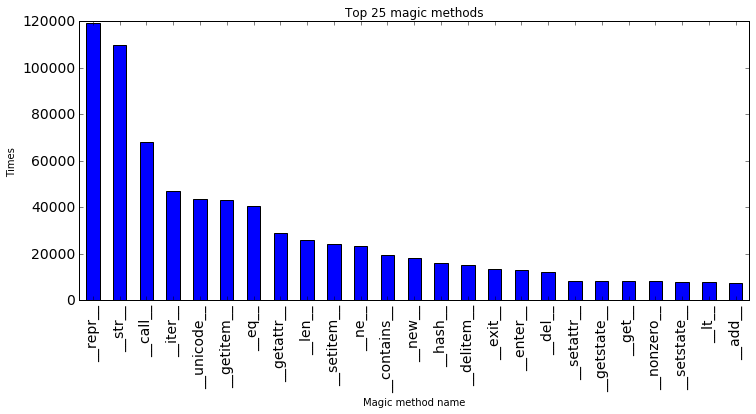
\includegraphics[width=82mm]{img/magic_methods.png}
\caption{Most common magic methods (\_\_init\_\_ not included).}
\label{fig:magic_ranking}
\end{figure}

As can be seen from Figure~\ref{fig:magic_ranking}, \_\_repr\_\_ and \_\_str\_\_ are the two most frequent magic methods. The next ones are: \_\_call\_\_ that implements a function call operator, \_\_iter\_\_ to create iterators, and \_\_unicode\_\_ which in Python 2 returns characters as \_\_str\_\_ really returns bytes\footnote{In Python 3, the \_\_str\_\_ magic method returns characters as in Python's 2 \_\_unicode\_\_, and a new \_\_bytes\_\_() magic method exists.}.


\section{Work in progress}

From all the repositories analyzed, we have extracted some information about the importance of Pythonic idioms. Right now, we are developing the web application that will allow to improve the knowledge in Pythonic idioms to anyone.

The application is running over Django, a high level Python framework that encourages rapid development and clean, pragmatic design\footnote{https://www.djangoproject.com/}.

When a user enters his username of GitHub in the web application, we select his profile repositories in a first approach and let him introduce others that he has contributed to. When the repositories are cloned, the tool filters the Python files looking at the extension or the first line of code.

Our work in progress is to identify the level of a user and give a mark about his Python knowledge. Our first approach is to classify the idioms in three different levels depending on the difficulty to be learnt.

For example, analyzing a previous version of the tool that extracts Pythonic idioms, we got the mark that is in figure ~\ref{fig:mark_pythonic}. That is a good mark, but is also tricky, because in this repository there are test for each idiom in Python.

\begin{figure}[ht]
\centering  
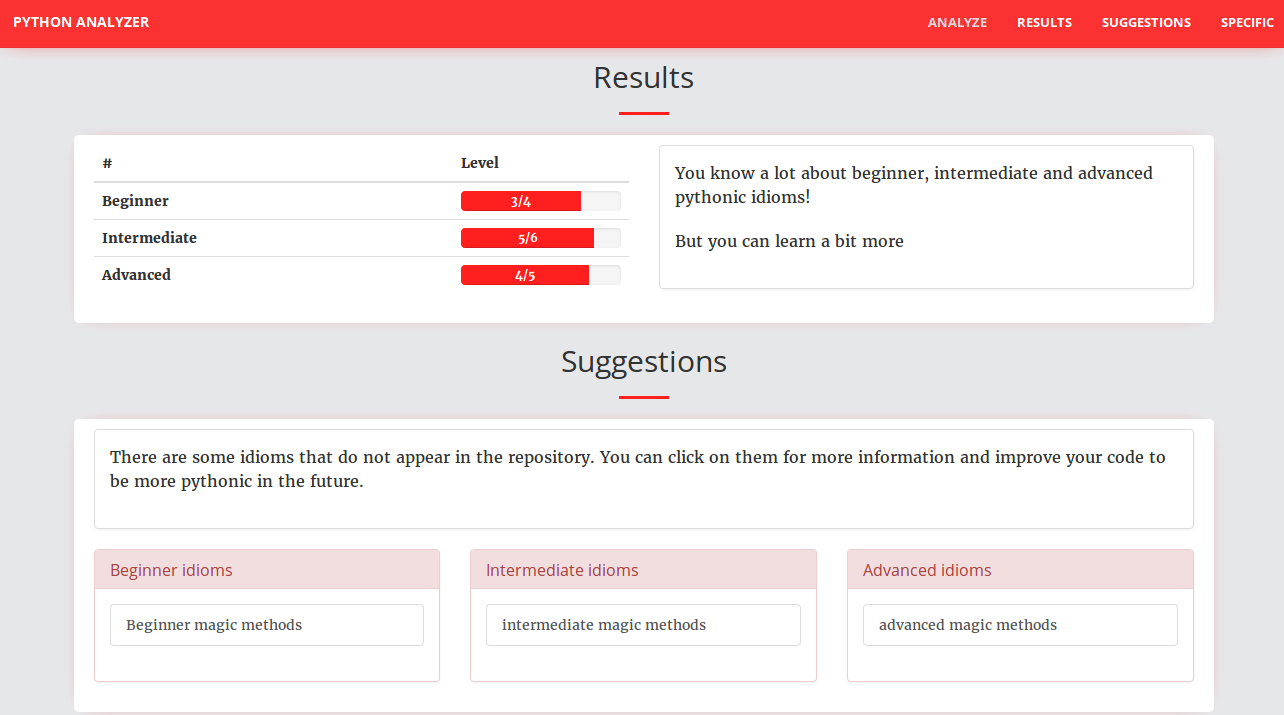
\includegraphics[width=82mm]{img/results_pythonic.png}
\caption{Results of 'Pythonic analyzer' repository}
\label{fig:mark_pythonic}
\end{figure}

We are working on better metrics that adjust better to the reality and by this way, assign a developer a level of mastery in the Python language and some path to improve his level.


\section{Future work}

This paper shows work-in-progress in our quest for finding how idioms are used in Python. In the near future, we would like to do the following:

\begin{itemize}

  \item Extend and assess the list of Python idioms. We would like to have a list of idioms as complete as possible. These should be evaluated by Python developers.
  
  \item There are idioms that are conceptually more difficult than others. We would like, again with the help of Python developers, see if we can classify the idioms by their complexity.
  
  \item If idioms are \emph{good} practices, we have noticed as well the existence of \emph{anti-idioms} (similar to the patterns and anti-patterns idea~\cite{brown1998antipatterns}). We would like to identify them and see how often they are used.
  
  \item We would like to filter projects by their importance, first by omitting pet or student projects (for instance those that have a lifetime of less than 6 months) and second by giving a weight to projects by using data from the Python Package Index (PIP).
  
  \item We would like to study how Python idioms get propagated. This has two perspectives: how do new Python idioms propagate, and how do developers learn them.

\end{itemize}

\section{Acknowledgements}

The work of Gregorio Robles has been funded in part by the Region of Madrid under project ``eMadrid - Investigaci\'on y Desarrollo de tecnolog\'ias para el e-learning en la Comunidad de Madrid'' (S2013/ICE-2715) and in part by the Spanish Government under project SobreVision (TIN2014-59400-R).


\bibliographystyle{abbrv}
\bibliography{references}


\end{document}
